\begin{frame}
\frametitle{Hardware used in this training session}
  Using BeagleBone boards in most practical labs
  \begin{columns}
    \column{0.7\textwidth}
    \begin{itemize}
        \item 720MHz super-scalar ARM Cortex-A8 (armv7a)
        \item 3D graphics accelerator
        \item ARM Cortex-M3 for power management
        \item 2x Programmable Realtime Unit 32-bit RISC CPUs
        \item USB client: power, debug and device
        \item USB host
        \item Ethernet
        \item 2x 46 pin headers: 2x I2C, 5x UART, I2S, SPI, CAN, 66x 3.3V GPIO, 7x ADC
    \end{itemize}
    \column{0.4\textwidth}
    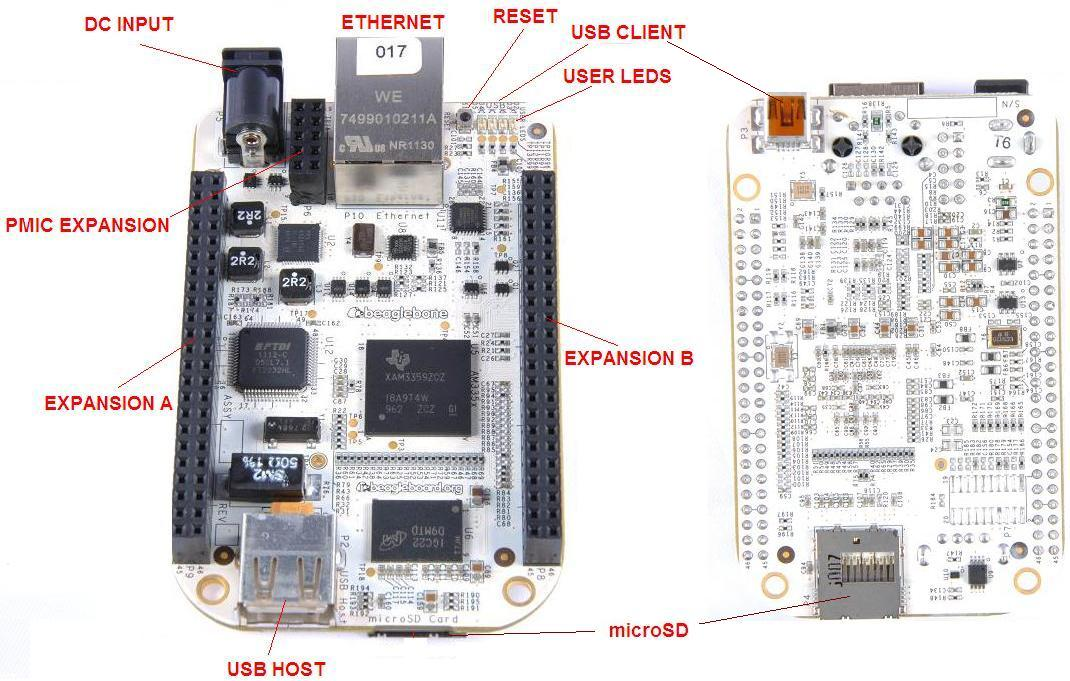
\includegraphics[width=\textwidth]{slides/beaglebone-board/beaglebone-board.jpg}
  \end{columns}
\end{frame}
